
\section{Computing for Energy Frontier Science}

Computing for experiments at the ``Energy Frontier'' (EF) is now dominated by
the huge data processing and analysis demands for the Large Hadron Collider
(LHC). The scale of the LHC computing problem has required to put in place the
global computing infrastructure of the LHC computing grid, which has been
hugely successful.  The LHC has driven much of the progress toward the
usability of a truly distributed computing environment, that makes full use of
networks to connect a tiered system of computing centers at various scales, to
federate storage systems enabling access to and analysis of hundred-petabyte-
scale data sets, and allowing to share the use of resources across different
science groups, thereby increasing overall throughput and productivity.

Progress in distributed high-throughput computing, in high-performance
networks, in distributed data management, in remote data access, in work flow
systems, etc, enables the experiment groups to marshal these diverse and
distributed resources into coherent systems, for production teams to run
immense data processing, management, simulation and distribution work flows,
and for a community of thousands of scientists to perform data analysis.
Collaboration is an important factor in this success. The Worldwide LHC
Computing Grid (WLCG)  and national Grid consortia were formed. In the U.S.
the Open Science Grid is  bringing together sites, experiments, infrastructure
provider and computing specialists, which is necessary for  sustaining and
further developing this distributed environment.

Today LHC computing routinely uses 250,000 CPU processor cores and nearly 170
petabytes of disk storage in addition to large multi-hundred petabyte capacity
tape libraries.  The experiments generate over a petabyte per second of data
at the detector device level. Triggering and real-time event filtering  is
used to reduce this by six orders of magnitude. In the case of LHC experiments
at the start of Run 2 this makes for a final rate to persistent storage of
around one gigabyte per second. The main requirement dictating the rate to
storage is keeping the storage cost, and the  cost of the computing to analyze
the stored data, at a tolerable level.

Looking forward, the HL-LHC stands out as a significant challenge, while
science at EF lepton colliders is unlikely to be constrained by computing
issues.  At the LHC, however, the expected increases in trigger rate, pileup
and detector complexity (number of channels) could increase the data rates by
a about a factor of 10 or more.   This order of magnitude increase in storage
and CPU requirements presents a new challenge for the computing infrastructure
and the community will need time to prepare for it. The LHC community is
beginning to review their computing models as they make plans for the next
decade.  It is anticipated that the general design will be an evolution from
the current models with the computing resources distributed at computing
centers around the world.

The full report on Computing for the EF bases its  prediction of the magnitude
of changes that should be expected over the coming 10 years, by looking back
on  the changes between the Tevatron and LHC over the past 10 years. We argue
that  the resource need increases for LHC Run2, starting in 2015 and ending
in 2021 with the possible start of  the HL-LHC upgrade, can probably be
accommodated with a roughly flat budget profile. However, the change to HL-LHC
will be a large disruptive step, like the one going from the Tevatron to the
LHC.

The increase in LHC computing and disk storage since its start is shown in
Figure~\ref{fig:growth}.  The CPU increases at a rate of 363kHS06 per year and
the disk at 34PB a year on average.  The rough linear increase is the
combination of three separate periods that average to linear.  The period
2008, 2009, and 2010 were the procurement ramp for LHC as the scale of the
available system was tested and commissioned. The period from 2010 to 2013 is
the first run where the computing and storage increased at a rate defined by
the incoming data to process and analyze.  The resources needed to accommodate
the higher trigger rate and event complexity expected in the second run define
2015.  The three periods roughly average out to a linear increase.

The growth curves below do not scale with total integrated luminosity but
indicate that more inputing is needed per unit time as trigger rates and event
complexity increase. It is not reasonable to expect that the techniques
currently used to analysis data in the EF will continue to scale indefinitely.
The EF will need to adopt new techniques and methods moving forward.

%%%%%%%%%%%%%%%%%%%%%%%%%%%%%%%%%%%%%%%%%%%%%%%%%%%%%%%%%%%%%%%%%%%%%%%%%
%%
%%   use this format to include an .pdf figure into your paper
%%
\begin{figure}[htb]
\begin{center}
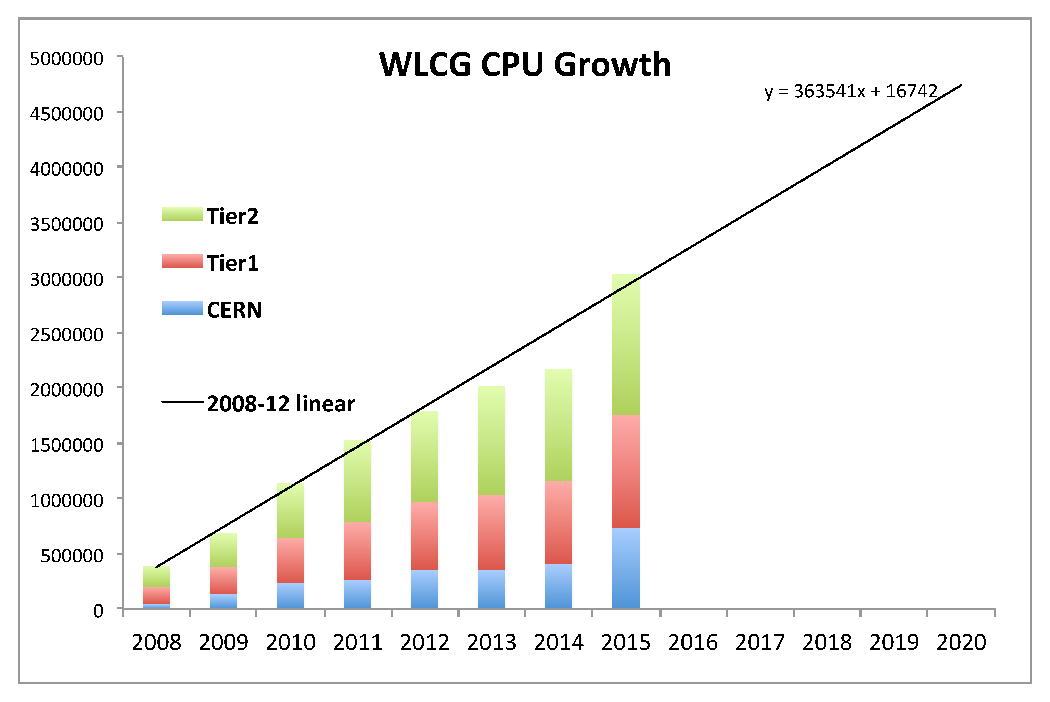
\includegraphics[width=0.45\hsize]{CpF-E2/Growth1.eps}
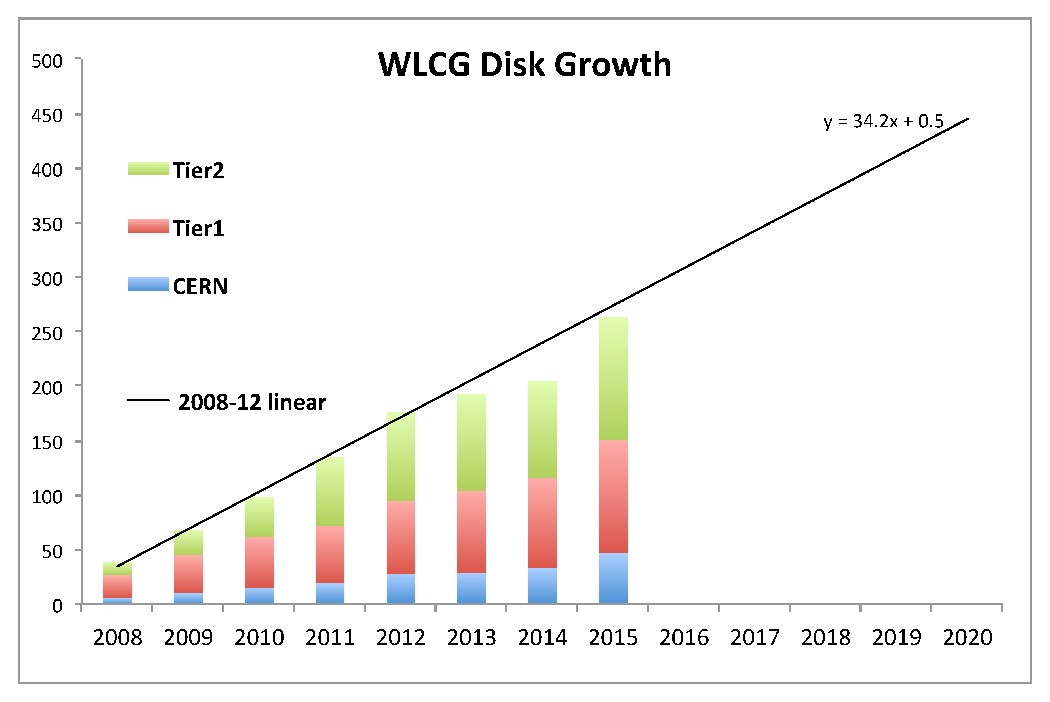
\includegraphics[width=0.45\hsize]{CpF-E2/Growth2.eps}
\caption{Shows the CPU and disk growth through the first 7 years of the program.}
\label{fig:growth}
\end{center}
\end{figure}
%%%%%%%%%%%%%%%%%%%%%%%%%%%%%%%%%%%%%%%%%%%%%%%%%%%%%%%%%%%%%%%%%%%%%%%%%%%


Using those cures to extrapolate out 10 years,  LHC computing would have
roughly 3 times the computing expected in 2015, which is lower than the
Moore's law doubling expectations.  LHC would reach nearly 800PB of disk by
2023, which again is roughly a factor of 3 over 2015.   These increases could
probably be achieved with close to flat budgets.   There are potential
efficiency improvements and new techniques that will be discussed below.

However, going to the HL-LHC or other proposed hadron collider programs,  the
luminosity and complexity increases dramatically and computing would not be on
the curve in Figure~\ref{fig:growth}, but would require a significant shift.
To estimate the resource needs going from the LHC to the HL-LHC the transition
from the Tevatron to the LHC is instructive.  We observe that in the 10 years
going from Tevatron in 2003 to LHC at the end of Run1,  the data rates are
about a factor of ten larger. However,  during that time the total computing
capacity went up by a factor of thirty,  and the disk capacity, the local data
served, the wide area networking from the host lab, and the inter-site
transfers all increased by a factor of 100 to accommodate this step.  The step
from LHC Run2 to the HL-LHC will similarly require very significant additional
resources, and quite possibly a disruptive change in technologies and
approaches to enable the large resource increase by  making better use of
resources. We identify two trends that will potentially help with this: the
increased use of specialized hardware, and providing and using computing as a
service.

On the one side the EF will need to evolve to use alternative computing
architectures and platforms like GPUs and other co-processors,  low-power
``small'' cores, etc, as the focus of industry development is moving away from
the classic server CPU.  Using GPUs introduces significant diversity to the
system, complicates the programming, and changes the approaches used in
scientific calculation, but can increase performance by orders of magnitude
for specific types of calculations.  Co-processors have similar potential
improvement gains, but also increase the diversity and complexity of the
system, and pose additional programming challenges.  Low power mobile
platforms are most interesting when they are combined into massively parallel,
specialized system where a single box may have the same number of cores as a
remote computing center does today.  These systems would be used more like a
super computer and less like a batch farm, which will require the field to
grow expertise in such much more interconnected computing environments.

Specialized hardware and architectures is likely to be deployed initially in
extremely well controlled environments, like trigger farms and other dedicated
centers, where the hardware and be controlled and specified. The next phase is
likely to be schedulable dedicated specialized systems to permit large-scale
calculations to achieve a goal similar to making a super computer center
request.  Large scale clusters of specialized hardware owned by the experiment
are likely to come last, and are only likely to come if they can completely
replace a class of computing resources and perform a function at a reduced
cost and higher efficiency.

The other trend impacting EF computing is the move to computing as a service
and other ``cloud'' solutions.  Currently,  commercial offerings, academic
resources, and opportunistic resources are all being offered through cloud
provisioning techniques.  While commercial solutions are still more expensive
than well used dedicated resources, there is a steady decrease in the pricing.

EF computing should expect a transition to more shared and opportunistic
resources provided through a variety of interfaces, including cloud
interfaces.   Effort is needed to allow the community to make effective use of
the diverse environments and to perform resource provisioning across
dedicated, specialized, contributed, opportunistic, and purchased resources.

There are considerable concerns regarding the enormous increase  in data
produced by the next round of EF colliders,   to be ingested by the offline
computing systems.  We observe that while the EF processing capacity has
increased largely with what would be expected from Moore's law and relatively
flat budgets, the storage requirements have grown much faster.  The larger
number of sites and the need for local caches, the increase in trigger rates,
and the larger event sizes drives the need for disk-based storage.

For EF discovery physics and searches there is a case for storing all
potentially interesting events, and then computationally  applying various
hypotheses to look for new physics.  For some searches and many measurements a
new approach where much more of the processing and analysis is done with the
initial data collection and only synthesized output is archived has the
potential for preserving physics while reducing the offline processing and
storage needs.  Already the ALICE experiment is planning to do mostly online
reconstruction starting with  the coming running period.   For experiments at
future EF accelerators there will be strong motivations to reconstruct and
calibrate online and write only constants.

We expect a change of mentality, moving away from the approach  that a higher
trigger rates are always better, and that all data from  all triggered events
need to be kept.   As the EF trigger rates go up by an order of magnitude,  as
expected for LHC running, and certainly for the HL-LHC,  the experiments
should expect to be more selective in what classes of events to fully
reconstruct,  and instead develop an approach of on-demand reconstruction,
calibration, and analysis.

Simulation and raw-data reconstruction produce  derived data and that can
entirely be reproduced. At the LHC, already many of the intermediate steps are
treated as transient data.   More of the data analysis steps should be moved
into the production chain, only keeping the final output, with the
understanding that it can be re-derived if required later.

With the expected increased diversity of computing resources, EF computing
needs to develop a data management system that can deal with all kinds of
resources.   In the next decade computing processing for the EF will evolve to
be less deterministic, with more emphasis on cloud provisioned resources,
opportunistic computing, local computing, and volunteer computing.   A data
management system that handles the placement of the data and allows the
operations team and analysis users to concentrate more on execution of work
flows and less on placement and location of data is needed.

Industry has put a focus on delivering content either through CDNs (Content
Delivery Networks)  or through peer-to-peer systems.  The experiment data
management systems need to evolve to be much less deterministic as well, in
order to make efficient use of the diverse landscape of resources that the
experiment computing models will have to adapt to.

The development of a data intensive content delivery network should not be
unique to one experiment, and should even be applicable to several scientific
domains, but will require commitment and effort to develop.


